\documentclass[11pt]{article}

% For ACL-family venues, replace the preamble with the official style:
%   \usepackage[review]{acl}
% and download acl.sty + acl_natbib.bst from the ACL template repository.
% For NeurIPS workshops, use the workshop's own style file instead.

\usepackage[margin=1in]{geometry}
\usepackage[T2A,T1]{fontenc}
\usepackage[utf8]{inputenc}
\usepackage[russian,english]{babel}
\usepackage{times}
\usepackage{graphicx}
\usepackage{booktabs}
\usepackage{amsmath}
\usepackage{url}
\usepackage[hidelinks]{hyperref}

\newcommand{\ky}[1]{\foreignlanguage{russian}{#1}}

\title{What LLMs Know About Kyrgyz and What They Cannot Do:\\
A Native-Authored Benchmark Separating Knowledge from Grammar}

\author{
  Yryskeldi Barpygulov \\
  \texttt{yrys.barpygulov@gmail.com}
}

\date{}

\begin{document}
\maketitle

\begin{abstract}
Kyrgyz, a Turkic language with roughly five million speakers, is nearly absent from
large language model evaluation. Where low-resource Turkic languages are measured at
all, the evidence is usually a translation score on a machine-translated test set,
which conflates the model with the translation system used to build the test.
We introduce a native-speaker-authored benchmark of 64 four-option items across eight
linguistic phenomena, from vowel harmony and agglutinative suffix stacking to idioms,
orthography, and culturally grounded knowledge. Scoring is deterministic and every
result is tested against a 25\% random baseline. Evaluating two frontier models we
find a consistent \emph{knowledge--grammar dissociation}: they answer factual and
lexical questions at or near ceiling (idioms, translation, and lexical semantics reach
100\%) while dropping to 62\% on the questions that require producing correct
morphology, with an identical score for the small and the large model in the family.
A 300-item, corpus-grounded morphology benchmark confirms the effect at scale
(gpt-4o 82.7\%, gpt-4o-mini 65.7\%). We then show the gap is learnable rather than
intrinsic: a rule engine for Kyrgyz nominal inflection, verified against the
hand-authored items, generates training data on which a 0.5B open model rises from
0\% to 77\% at producing inflected forms for held-out words. We release the benchmark,
the rule engine, and all code.
\end{abstract}

\section{Introduction}
\label{sec:intro}

Multilingual evaluation of large language models is concentrated on a small set of
high-resource languages. For the Turkic family, and for Kyrgyz in particular,
published evidence of competence is thin and mostly indirect. The usual number is a
translation score computed on a human- or machine-translated test set such as
FLORES-200 \cite{nllb2022}. Such a score conflates two systems: it rewards the model
for the parts
of the sentence the translation pipeline happened to render well, and it says nothing
about whether the model can produce a grammatical Kyrgyz form on demand.

A deeper problem is that a single aggregate accuracy hides \emph{which} competence a
model has. ``90\% on Kyrgyz'' could mean the model handles the language well, or it
could mean the model knows many facts stated in Kyrgyz while being unable to inflect a
noun. These are very different capabilities, and only the second is what a speaker
would call knowing the grammar. Distinguishing them requires items that target
individual phenomena and a task on which guessing does not pay.

We build such a benchmark for Kyrgyz. Every item is written and verified by a native
speaker rather than translated, and each targets one phenomenon a model without real
Kyrgyz competence should fail: vowel harmony, agglutinative suffix stacking, syntax,
lexical semantics, idioms, culture, translation, and the orthography of the
Kyrgyz-specific letters \ky{ң}, \ky{ө}, \ky{ү}. Items are four-option multiple choice,
so scoring is exact and every result can be tested against a 25\% baseline.

Our contributions are:
\begin{itemize}
  \item A native-authored Kyrgyz benchmark of 64 items across eight phenomena, with
        balanced answer positions and per-item explanations.
  \item An evaluation of frontier models showing a \emph{knowledge--grammar
        dissociation}: near-ceiling factual accuracy alongside a sharp and
        scale-invariant drop on morphology.
  \item A rule engine for Kyrgyz nominal inflection, verified against the
        hand-authored items and cross-checked against an independent finite-state
        description, that generates unlimited training and test data from
        corpus-attested stems.
  \item A fine-tuning study showing the morphological gap is learnable: open models
        go from 0\% to the mid-70s at producing inflected forms for unseen words, and
        the benefit grows with base-model size.
\end{itemize}

\section{Related Work}
\label{sec:related}

\paragraph{Multilingual evaluation and language coverage.}
Massively multilingual benchmarks such as XTREME \cite{hu2020xtreme} and
MEGAVERSE \cite{ahuja2024megaverse} evaluate models across dozens of languages, but
their coverage of any individual low-resource language is thin, and much of the
non-English data is obtained by translation rather than native authoring. Knowledge
benchmarks in the MMLU family \cite{hendrycks2021mmlu} have been extended to more
languages largely through machine translation, which can introduce errors and misses
culturally specific content. Our benchmark is deliberately narrow and native: one
language, eight phenomena, every item written by a speaker.

\paragraph{Turkic and Kyrgyz resources.}
The closest work is TUMLU \cite{tumlu2025}, a native, MMLU-style understanding
benchmark spanning nine Turkic languages including Kyrgyz. TUMLU measures
subject-matter knowledge expressed in these languages; we instead isolate grammatical
competence, and in particular the production of morphology, which subject-matter
questions do not test. For Kyrgyz specifically the main existing resources are the
Universal Dependencies treebanks \cite{nivre2020ud}, which we use as one source of
attested nouns, and the Apertium finite-state description
\cite{forcada2011apertium,khanna2021apertium}, whose morphological rules we use both
as a stem source and as an independent check on our own rule engine.

\paragraph{Morphological inflection.}
The SIGMORPHON shared tasks \cite{mccarthy2019sigmorphon,vylomova2020sigmorphon}
established inflection generation from a lemma and morphosyntactic features as a
standard evaluation, across typologically diverse and often low-resource languages.
Our generation task is in that tradition, but the object of study is different: rather
than building the best inflection system, we ask whether a general-purpose LLM can
inflect at all, and whether targeted data repairs the deficiency.

\paragraph{Data augmentation for low-resource morphology.}
A recurring finding in that literature is that synthetic data, in particular the
``hallucination'' of new stems, sharply improves low-resource inflection
\cite{anastasopoulos2019inflection}. Our rule engine is a deterministic instance of
the same idea: because Kyrgyz nominal morphology is rule-governed, we can generate
correct training pairs for arbitrarily many attested stems rather than sampling them,
and we use them to teach the phenomenon rather than to win a shared task.

\paragraph{Translation benchmarks and dictionaries.}
Human-translated evaluation sets such as FLORES-200, released with NLLB
\cite{nllb2022}, are the usual way low-resource languages enter LLM evaluation; they
measure translation quality, which conflates the model with the translation setup and
does not probe morphology directly. For lexical resources we draw on Wiktionary via
the Wiktextract pipeline \cite{ylonen2022wiktextract}.

\section{Benchmark Construction}
\label{sec:benchmark}

\subsection{Categories}

The benchmark covers eight categories, chosen so that failure in each isolates a
different competence (Table~\ref{tab:categories}). Four are broadly about knowledge
of the language (lexical semantics, idioms, culture, translation) and four about its
form (vowel harmony, morphology, syntax, orthography).

\begin{table}[h]
\centering
\small
\begin{tabular}{ll}
\toprule
Category & Tests \\
\midrule
Vowel harmony      & suffix vowel required by the stem \\
Morphology         & case, possessive, number stacking \\
Syntax             & well-formedness of a sentence \\
Lexical semantics  & word meaning, synonymy \\
Idioms             & non-literal fixed expressions \\
Culture            & Kyrgyz-specific knowledge \\
Translation        & meaning across ky/ru/en \\
Orthography        & \ky{ң}, \ky{ө}, \ky{ү} and similar \\
\bottomrule
\end{tabular}
\caption{Benchmark categories. Eight items each; 64 in total.}
\label{tab:categories}
\end{table}

\subsection{Authoring protocol}

Items were written directly in Kyrgyz by a native speaker, not translated or scraped.
Each item has a question, four options, a marked correct answer, and a short English
explanation of why that answer is correct; the explanations are the basis for the
error analysis in Section~\ref{sec:analysis}. The guiding rule for distractors is that
each must be a mistake a learner or an under-trained model would plausibly make, such
as a form with the wrong vowel-harmony class, rather than obvious nonsense that could
be eliminated without knowing Kyrgyz.

\subsection{Annotator agreement}

TODO: report inter-annotator agreement over the answer keys with at least two
additional native speakers (Cohen's $\kappa$ for two, Fleiss' $\kappa$ for more).
This is currently the largest methodological gap and the first thing a reviewer will
look for.

\subsection{Design controls}

Each item has exactly four distinct options and a validated answer key; a validation
script enforces both. Because a model that always selects one position would beat
chance on a skewed set, the position of the correct answer is balanced to exactly
25\% per slot in the core benchmark, and the script reports the distribution so any
imbalance is visible.

\section{Experimental Setup}
\label{sec:setup}

\paragraph{Models.} We evaluate \texttt{gpt-4o} and \texttt{gpt-4o-mini} \cite{openai2023gpt4} on the core
benchmark. The fine-tuning study additionally uses the open models
\texttt{Qwen2.5-0.5B-Instruct} and \texttt{Qwen2.5-3B-Instruct} \cite{qwen2025}.
TODO: fix exact model version strings and access dates, and add further frontier
models (for example Gemini and Claude) to show the dissociation is not specific to one
provider.

\paragraph{Prompting.} Items are presented in Kyrgyz with numbered options and the
model is asked to reply with a single digit. Numeric labels rather than A/B/C/D avoid
Latin/Cyrillic homoglyph ambiguity between \texttt{A} and \ky{А} in the reply.

\paragraph{Scoring.} A reply is parsed to an option index, first by a bare digit and
then by exact match against option text. Replies yielding neither are recorded as
\emph{unparseable}, counted as incorrect, and reported separately, since a model that
cannot follow the instruction fails differently from one that answers wrongly.

\paragraph{Statistics.} Accuracy is compared against the 25\% chance level with a
one-sided binomial test, overall and per model $\times$ category, and we report Wilson
95\% confidence intervals on the larger morphology set.

\section{Results}
\label{sec:results}

Both models score well overall on the core benchmark
(Table~\ref{tab:overall}), far above the 25\% baseline. The overall number, however,
is exactly what hides the effect of interest.

\begin{table}[h]
\centering
\small
\begin{tabular}{lrr}
\toprule
Model & Accuracy & $p$ vs.\ chance \\
\midrule
gpt-4o       & 59/64 (92.2\%) & $6\times10^{-30}$ \\
gpt-4o-mini  & 55/64 (85.9\%) & $2\times10^{-24}$ \\
\bottomrule
\end{tabular}
\caption{Overall accuracy on the 64-item core benchmark. Chance is 25\%.}
\label{tab:overall}
\end{table}

Breaking the score down by category (Figure~\ref{fig:heatmap}) reveals a sharp split.
The knowledge categories are at or near ceiling: idioms, lexical semantics, and
translation are 100\% for both models, and culture is 100\% for gpt-4o. The form
categories are much lower and, crucially, do not improve with model size within the
family: morphology is 62\% for \emph{both} gpt-4o and gpt-4o-mini, and vowel harmony
is 75\% for both. Scaling from the small to the large model, which lifts the knowledge
categories, buys nothing on morphology.

\begin{figure}[h]
\centering
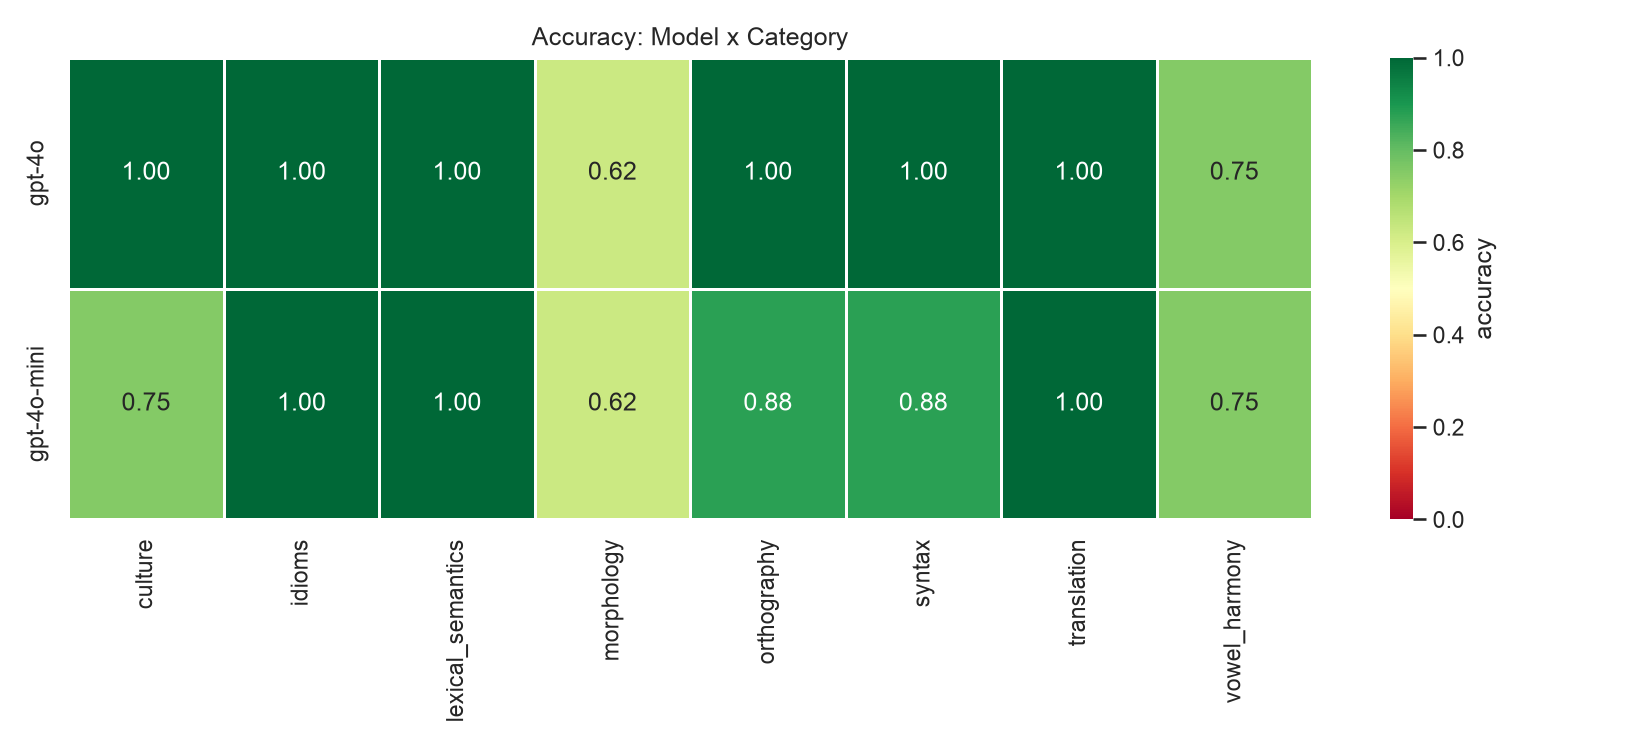
\includegraphics[width=\columnwidth]{../results/report/model_category_heatmap.png}
\caption{Accuracy by model and category on the core benchmark. Knowledge categories
are near ceiling; morphology and vowel harmony are the floor and do not rise with
scale.}
\label{fig:heatmap}
\end{figure}

\paragraph{The effect holds at scale.} Eight items per category is a small basis for
a claim, so we built a second, morphology-only benchmark of 300 items whose stems are
real nouns attested in independent corpora (Section~\ref{sec:data}) and whose answers
come from the verified rule engine. On this larger set the drop is confirmed with tight
confidence intervals: gpt-4o scores 248/300 (82.7\%, 95\% CI 78--87\%) and gpt-4o-mini
197/300 (65.7\%, 95\% CI 60--71\%). The per-case breakdown
(Figure~\ref{fig:byfeature}) is itself informative and is analysed below.

\begin{figure}[h]
\centering
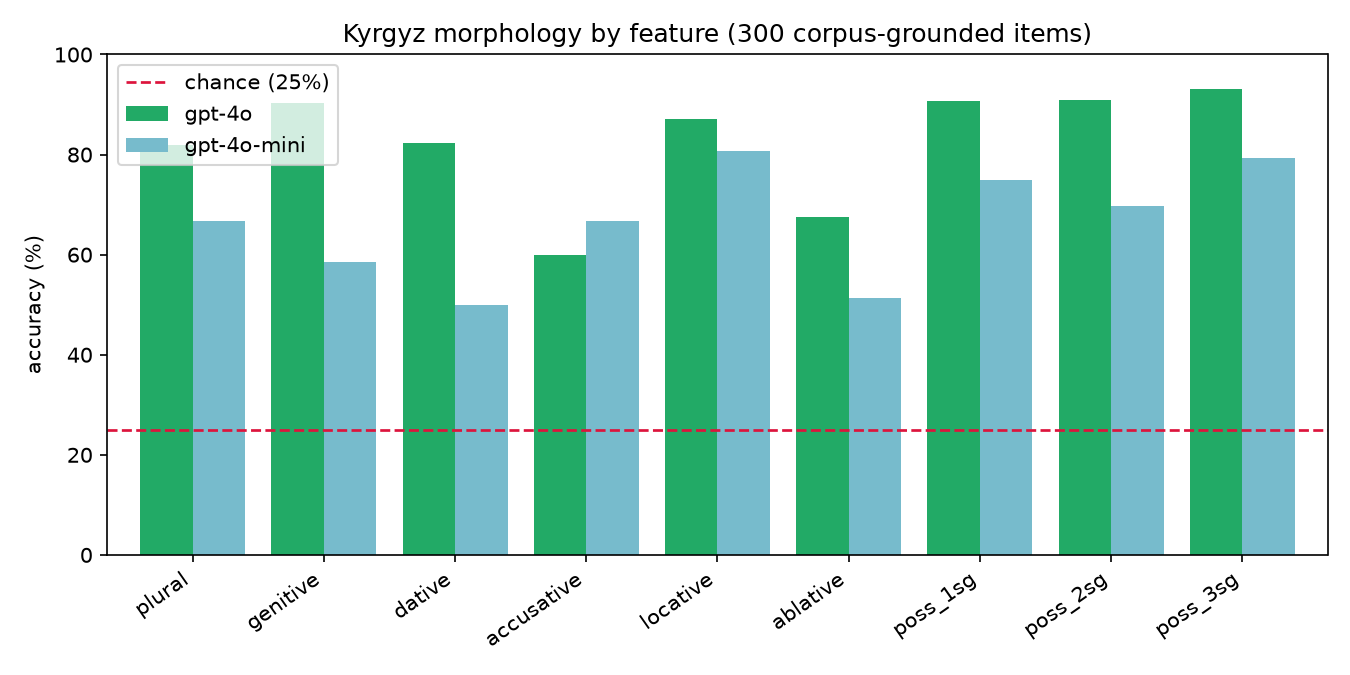
\includegraphics[width=\columnwidth]{../results/report/generated_by_feature.png}
\caption{Accuracy by inflectional feature on the 300-item corpus-grounded morphology
benchmark. Both models are weakest on the ablative and accusative; possessives, whose
suffix is more regular, are strongest.}
\label{fig:byfeature}
\end{figure}

\section{Analysis}
\label{sec:analysis}

\subsection{The knowledge--grammar dissociation}

The models know a great deal \emph{about} Kyrgyz while being unable to reliably
\emph{produce} it. Retrieval-style categories, where the answer is a memorised fact or
a lexical association, are at ceiling; generative morphology, where the answer must be
computed from the stem by phonological rule, is far lower and flat across scale. A
single aggregate score conceals this because most of the questions a broad benchmark
asks reward the first ability. The practical implication is that reported multilingual
scores can substantially overstate a model's command of a low-resource language's
grammar.

\subsection{Which morphology is hard}

The per-case results sharpen the picture. Both models are weakest on the cases whose
suffix must both harmonise in vowels and assimilate in its onset consonant to the
stem: the ablative and the accusative sit near 60\% even for gpt-4o. The possessives,
whose suffix is comparatively regular, reach the low 90s. The gap between the small and
large model is widest exactly on the cases that demand the most phonological
computation (dative, genitive), which is where model scale appears to help most. The
weakness is therefore not uniform ``bad at morphology'' but tracks the amount of
rule-governed computation each form requires.

\subsection{Error typology}

The clearest single case is a form both models produced identically and incorrectly:
for \ky{дос} (`friend') with plural and first-person possessive, both answered
\ky{достарым} where the correct form is \ky{досторум}. The rounded vowel of the stem
requires rounded suffixes throughout the word, and both models default to the
unrounded series. More broadly the residual errors of the fine-tuned models concentrate
on two rules that interact with the stem-final consonant: intervocalic voicing (for
example a target \ky{-би-} realised as \ky{-пи-}) and devoicing of the suffix onset
after a voiceless stop. These are precisely the points where a form cannot be produced
by concatenation and requires a phonological alternation.

\section{A Rule Engine and Corpus-Grounded Data}
\label{sec:data}

\subsection{Rule engine}

We implement Kyrgyz nominal inflection as an explicit rule engine covering four-way
vowel harmony, three-way and two-way consonant assimilation of suffix onsets,
final-obstruent voicing, and the orthographic realisation of glide--vowel sequences.
One subtlety worth noting is that rounding harmony in low suffix vowels is asymmetric:
it is triggered by a mid rounded stem vowel (\ky{о}, giving \ky{жол}~$\to$~\ky{жолдор})
but not by a high one (\ky{у}, giving \ky{суу}~$\to$~\ky{сууга}, not \ky{сууго}). The
engine is unit-tested against the hand-authored benchmark forms, so generated data
inherits native-verified answers. During development the fine-tuned model repeatedly
disagreed with one class of gold forms; the disagreement turned out to be a bug in an
early version of our own rule, which the independent Apertium finite-state description
of Kyrgyz \cite{khanna2021apertium} confirmed, after which the rule was corrected. We
regard this as evidence for, not against, the reliability of the final engine.

\subsection{Stem selection}

Stems are drawn from three independent resources: the Apertium Kyrgyz morphological
dictionary \cite{khanna2021apertium}, the Universal Dependencies Kyrgyz treebanks
\cite{nivre2020ud}, and Wiktionary via Wiktextract \cite{ylonen2022wiktextract}. A
stem is kept only if at least two of the three attest it, which removes typos and one-off
dictionary artefacts, and the treebank token counts give a frequency ranking so the
selected stems are common words rather than an arbitrary sample. We further screen out
Russian borrowings using orthographic cues and, principally, the fact that a native
Kyrgyz root keeps all its vowels in one backness class, so a disharmonic word such as
\ky{коридор} is rejected while \ky{карышкыр} is kept. A final check removes lemmas that
are already plural. The surviving stems are balanced across all sixteen combinations of
vowel-harmony class and final-segment type so that no cell of the paradigm is starved.

\section{Closing the Gap by Fine-Tuning}
\label{sec:finetune}

\paragraph{Setup.} Stems are split so that test stems never appear in training; any
gain therefore reflects generalisation of the rules rather than memorisation of forms.
We fine-tune with LoRA \cite{hu2022lora} on the rule-generated training pairs and
evaluate two ways: a
\emph{generation} task, where the model must write the inflected form and it must match
exactly, and the four-option \emph{recognition} task used for the benchmark.

\paragraph{Generation.} Before training, both open models score 0\% at producing
inflected forms; they echo the stem unchanged. After training on the rule data the
0.5B model reaches 77.0\% and the 3B model 73.8\% on held-out words
(Table~\ref{tab:finetune}). The rules are genuinely learned and generalise to unseen
stems.

\paragraph{Recognition.} On the multiple-choice task the same fine-tuning helps but by
less, and a larger base benefits more: the 0.5B model moves from 29.3\% to 40.0\% and
the 3B model from 28.0\% to 47.0\% (Figure~\ref{fig:mcq}). The two tasks measure
different abilities. Generation, the setting of the SIGMORPHON inflection
tasks \cite{vylomova2020sigmorphon}, isolates whether the morphological rules have been
acquired; recognition additionally requires parsing a Kyrgyz question and weighing four
distractors, which is bounded by the broader language understanding a small model
lacks. This is why the fine-tuned open models still trail the frontier models on
recognition despite matching or exceeding nobody-inflects-at-all baselines on
generation, and why closing the recognition gap would require a larger base; the upward
trend from 0.5B to 3B suggests it is reachable.

\begin{table}[h]
\centering
\small
\begin{tabular}{lrr}
\toprule
Model & Generation & Recognition (MCQ) \\
\midrule
Qwen2.5-0.5B base          & 0.0\%  & 29.3\% \\
\quad + LoRA (rule data)   & 77.0\% & 40.0\% \\
Qwen2.5-3B base            & 0.0\%  & 28.0\% \\
\quad + LoRA (rule data)   & 73.8\% & 47.0\% \\
gpt-4o-mini (base)         & ---    & 65.7\% \\
gpt-4o (base)              & ---    & 82.7\% \\
\bottomrule
\end{tabular}
\caption{Fine-tuning on rule-generated data, evaluated on held-out stems. Generation
is exact-match production; recognition is the four-option benchmark. Frontier models
were run on recognition only.}
\label{tab:finetune}
\end{table}

\begin{figure}[h]
\centering
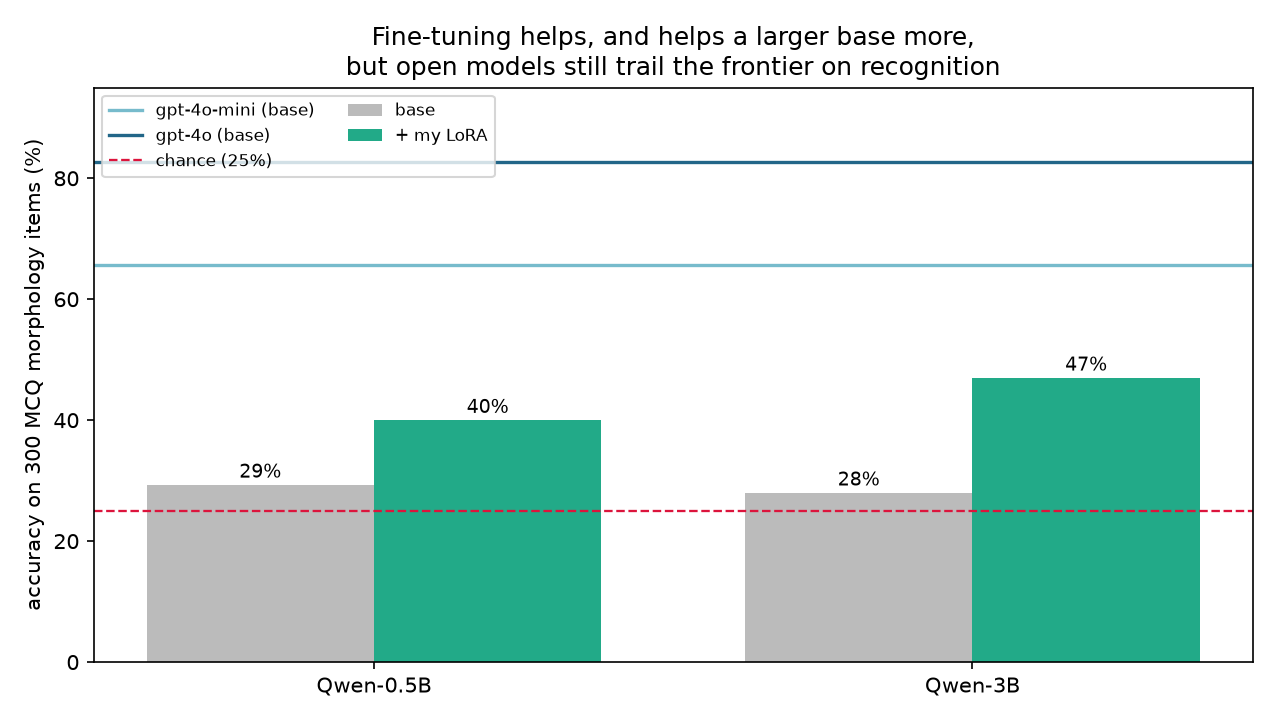
\includegraphics[width=\columnwidth]{../results/report/mcq_four_models.png}
\caption{Recognition accuracy on the 300-item morphology benchmark. Fine-tuning helps
both open models and helps the larger base more, but they still trail the frontier
models on this task.}
\label{fig:mcq}
\end{figure}

\section{Limitations}
\label{sec:limitations}

\begin{itemize}
  \item The core benchmark is small (64 items) and covers a single language.
  \item Multiple choice measures recognition, which is easier than free production;
        we therefore report generation separately in the fine-tuning study.
  \item Answer keys are currently authored by one native speaker; dialectal and
        prescriptive-versus-colloquial disagreement is possible, and inter-annotator
        agreement is not yet reported.
  \item The rule engine and the generated benchmark cover nominal morphology only.
  \item Compute constraints limited fine-tuning to models up to 3B; a frontier-scale
        open base is left to future work.
\end{itemize}

\section{Conclusion}
\label{sec:conclusion}

Evaluated on a native-authored, guessing-proof benchmark, frontier language models
know a great deal about Kyrgyz while failing to produce its morphology, and this gap
does not close with model scale within a family. A single aggregate score hides the
effect. The gap is nonetheless learnable: rule-generated data teaches an open model to
inflect held-out words from scratch. Measuring production, not just recognition or
translation, is what makes the deficiency visible and, ultimately, fixable.

\section*{Ethics and Data Statement}

All benchmark items were authored by a native speaker rather than scraped, and contain
no personal data. Stems are drawn from openly licensed resources. The benchmark, the
rule engine, and all code are released openly to support a language with few
computational resources.

\section*{Availability}

Code, benchmark, and rule engine:
\url{https://github.com/yryssqq/kyrgyz-llm-benchmark}

\bibliographystyle{plain}
\bibliography{refs}

\end{document}
